% This document is available under the Creative Commons Attribution-ShareAlike
% License; additional terms may apply. See
%   * http://creativecommons.org/licenses/by-sa/3.0/
%   * http://creativecommons.org/licenses/by-sa/3.0/legalcode
%
% Copyright 2010 Jérôme Pouiller <jezz@sysmic.org>
%

\part{Temps réel}

\begin{frame}
  \partpage
\end{frame}

\begin{frame}
  \tableofcontents[currentpart]
\end{frame}

\section{Problématique des OS RT} %(45min)

\begin{frame}{Contexte}
  Garantie qu'une action est éxecutée en moins d'un temps donné.

  Implique:
  \begin{itemize}
  \item Une garantie de qualité (0 bug)
  \item  Souvent  des  processus  garantissant  la  qualité  dans  les
    différentes phases: conception, développement, validation
  \item  Une  connaissances  importante de  l'environnement  extérieur
    (fréquence maximum des interruption, etc...)
  \end{itemize}
  $\to$ On se limitera à l'architecture logicielle
\end{frame}

\begin{frame}{Contexte}
  Ordonnancement statique:
  \begin{itemize}
    \item Charge des taches temps réelles $\ll 100\%$
    \item[$\to$]   Ordonnancement   avec   des   priorités   statiques
      suffisante
    \item[$\to$]  Problématique  des  algorithmes  d'ordonnancement  à
      priorité dynamique (EDF, LST, etc...) secondaire
  \end{itemize}
\end{frame}

% En d'autre termes:
\begin{frame}{Contexte}
  $$
  R_i = C_i + \sum_{j \in hp(i)} \left\lceil\frac{R_i}{T_j}\right\rceil C_j
  $$
  Pour les allergiques: le temps de  réponse d'une tâche est égal à la
  somme du temps d'exécution de la tache et de toutes les tâche de
  priorité supérieure qui s'exécutent en même temps.\\[1.5ex]
  Objectif: Rendre cette formule assez simple pour être prédictible.\\[1.5ex]
  Pas si simple:
  \begin{itemize}
  \item Interruptions
  \item Changement de contexte
  \item Sections critiques (ordonnanceur désactivé)
  \item Caches, Swap
  \end{itemize}
\end{frame}

% Schema des temps de réponses
% La principale chose que nous allons combattre, sera le temps de réponse aux
% évènements. Le temps de réponse peut-être très aléatoire
% Si on avait un temps de réponse null (ou au moins constant). Alors, il
% deviendrait simple de calculer les temps de réponse maximum de nos taches
\begin{frame}{Latence aux évènements}
  \begin{itemize}
  \item Coeur du problème
  \item  Si  la  latence  était   nul  (ou  au  moins  constante),  on
    calculerait simplement le temps de réponses de nos tâches.
  \end{itemize}

  \begin{center}
   \begin{tikzpicture}[scale=0.8]
     \tikzstyle{msize}=[main, minimum height=2cm, font=\LARGE]
     \draw
       node[anchor=south]                at (2, 3) {Interruption}
       edge[->, line width=0.5mm]  (2, 1.5)
       node[msize, cblue,  minimum width=4cm, text width=4cm] at (  0, 0) {Tache}
       node[msize, cgreen, minimum width=3cm, text width=3cm] at (3.5, 0) {Latence}
       node[msize, cblue,  minimum width=6cm, text width=6cm] at (  8, 0) {Tache de priorité supérieure}
       (-2, -1.2) edge[->, line width=0.5mm]  (11, -1.2)
       node at (10, -1.5) {temps};
   \end{tikzpicture}
  \end{center}
\end{frame}

\begin{frame}{Latence aux évènements}{Exemple concret}
  \begin{itemize}
  \item On paramètre un timer à 50Hz
  \item On mesure le temps effectif de chaque période
  \end{itemize}
\end{frame}

% Exemple concret
% Expliquer que l'on paramètre un timer à 50Hz
% On mesure les période effectives
% Le temps de réponse est ici très aléatoire et dépend fortement de la charge de la machine
% Schema des temps de réponses
\begin{frame}{Latence aux évènements}{Système classique}
  \begin{center}
    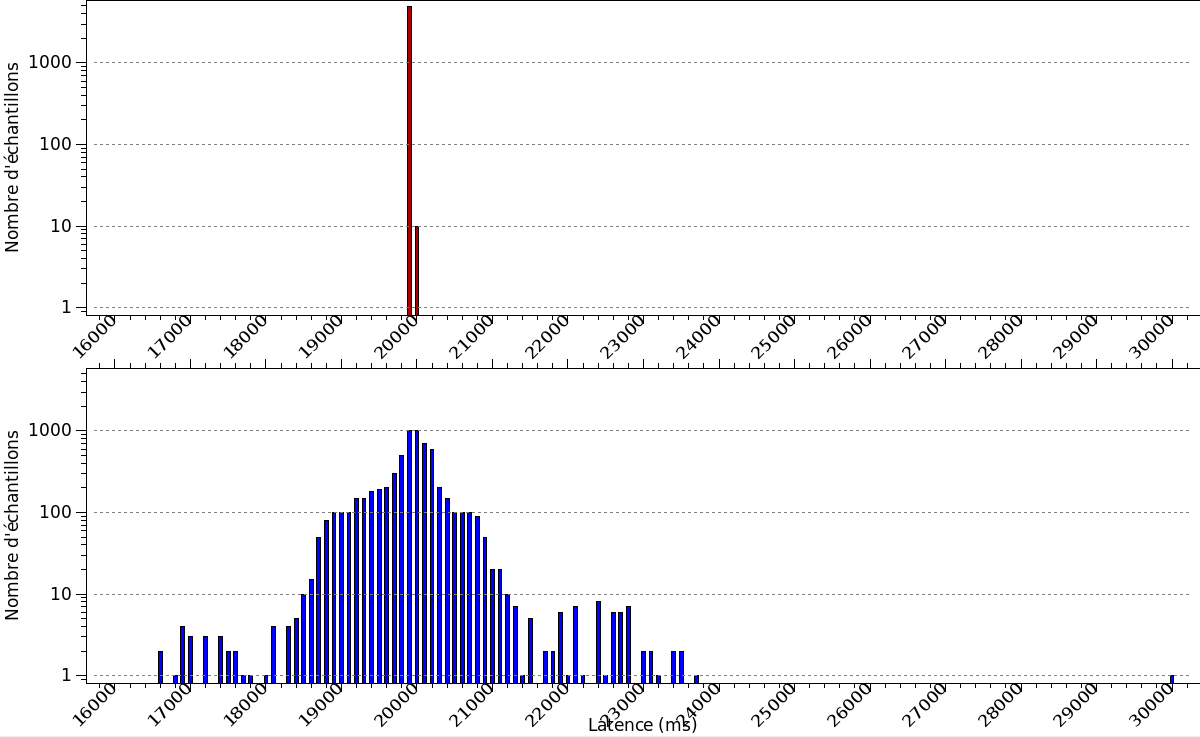
\includegraphics[width=\textwidth]{pics/latencyNorm}
  \end{center}
\end{frame}

% Le temps de réponse ici est beaucoup mieux borné
% Schema des temps de réponses
\begin{frame}{Latence aux évènements}{Système temps réels}
  \begin{center}
    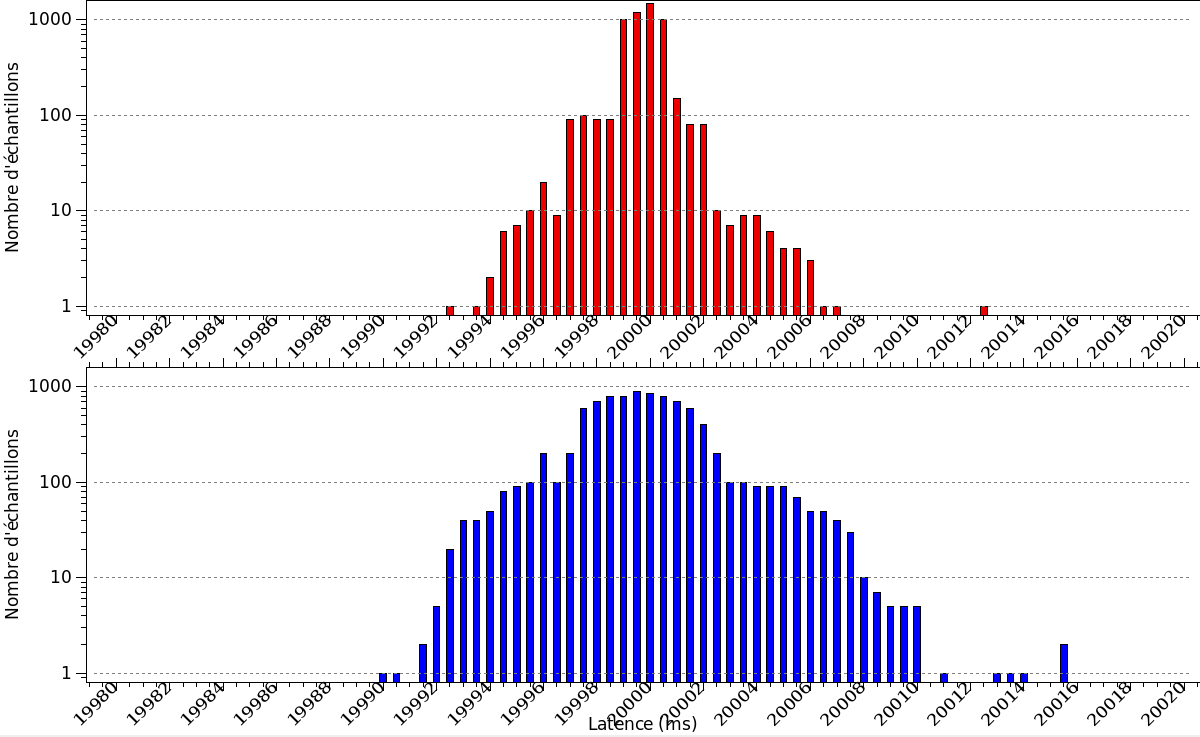
\includegraphics[width=\textwidth]{pics/latencyRT}
  \end{center}
\end{frame}

\begin{frame}{Tâches Posix}{Processus}
  \begin{columns}
    \begin{column}{3.5cm}
      \begin{tikzpicture}[scale=0.9]
     \filldraw[cbrown]
       (-2,-0.5) rectangle +(4,7);
     \draw 
       node[size2, cred]    at (0, 6) {Pile}
       node[size2, corange] at (0, 3) {Données mappées}
       node[size2, cyellow] at (0, 2) {Tas}
       node[size2, cgreen]  at (0, 1) {Données statiques}
       node[size2, cblue]   at (0, 0) {Code};
     \end{tikzpicture}
   \end{column}
   \begin{column}{6.5cm}
     \begin{itemize}
     \item Utilisation de la MMU
     \item[$\to$]    Permet    de    cloisonnement    des    processus
       (\emph{Multitâche})
     \item[$\to$] Permet de partage de pages (r--/rw-/r-x)
     \item Communication inter-processus (IPC) relativement complexe
     \item[$\to$] Noyau
     \item[$\to$] Pages partagées
       \note[item]({il faut mapper des morceau de memoire dans deux processus) ou passer par le noyau comme arbitre}
     \item Le noyau possède un contexte
     \item Le noyau est le seul à pouvoir modifier la MMU
     \end{itemize}
   \end{column}
  \end{columns}
\end{frame}


\begin{frame}{Tâches Posix}{Threads}
  \begin{columns}
    \begin{column}{3.5cm}
      \begin{tikzpicture}[scale=.9]
        \filldraw[cbrown] (-2,-0.5) rectangle +(4,7);
        \draw 
          node[size2, cred]    at (0, 6) {Pile thread 1}
          node[size2, cred]    at (0, 5) {Pile thread 2}
          node[size2, cred]    at (0, 4) {Pile thread 3}
          node[size2, corange] at (0, 3) {Données mappées}
          node[size2, cyellow] at (0, 2) {Tas}
          node[size2, cgreen]  at (0, 1) {Données statiques}
          node[size2, cblue]   at (0, 0) {Code};
      \end{tikzpicture}
    \end{column}
    \begin{column}{6.5cm}
      \begin{itemize}
      \item Même contextes
      \item[$\to$] Partage de la mémoire
        \item[$\to$] Échange de données facilité
          \note[item]{pas besoin de passer par le noyau pour communiquer}
        \item[$\to$] Posix offre pas mal de services   
        \item[$\to$] Moins de sécurité   
        \item Optimisations possible pour l'ordonnancement de threads
        \item[$\to$] Grouper l'ordonnancement des threads pour réduire
          les changement de contexte
        \item[$\to$]  Placer les  threads d'un  même processus  sur le
          même CPU pour réduire les erreurs de cache
      \end{itemize}
    \end{column}
  \end{columns}
\end{frame}

\begin{frame}{Tâches Posix}{Interruptions}
  \begin{itemize}
   \item Interruption matérielle: 
   \begin{itemize}
    \item Interrompt la tache en cours
    \item Gère l'interruption dans  le contexte noyau (+/- suivant les
      architectures et les types d'interruption)
    \item Le driver approprié fait son travail
   \end{itemize}
   \item Appel système (syscall):
   \begin{itemize}
   \item  Appel à  une fonction  du noyau  avec le  contexte  du noyau
     (exemple: envoi d'un packet réseau, ou sleep)
   \item  Techniquement,  on  déclenche  une  interruption  logicielle
     (historiquement, maintenant, ca s'optimise)
   \end{itemize}
  \end{itemize}
\end{frame}

\section{Le multitache}

\begin{frame}{Le monotache}{Par scrutation} 
  \begin{itemize}
    \item Une tache
    \item Difficulté d'extention 
    \item Difficulté d'implémentation si les fréquences de vérifications des capteurs sont différentes
    \item CPU utilisé de manière sous-optimale
    \item Latence peu controlée
  \end{itemize}
\end{frame}

\begin{frame}{Le monotâche}{Interruptions synchrones}
  \begin{itemize}
    \item Une tache
    \item ... + des interruptions
    \item Modèle MS-DOS
    \item Latence dans le cas de traitement dans l'interruption
  \end{itemize}
\end{frame}

\begin{frame}{Le monotâche}{Interruptions asynchrones}
  \begin{itemize}
    \item Traitement dans la tache principale
    \item Modèle de la plupart des logiciels des petits microcontrolleurs
    \item Pas de prioritisation des actions
    \item Partage d'informations entre les interruption et la tache
    \item[$\to$] Sections critiques
    \item[$\to$] Inhibition les interruptions
    \item Latence peu controlée
  \end{itemize}
\end{frame}

\begin{frame}{Evolution du multitache}{Multitache non-préemptif}
  \begin{itemize}
   \item Capacité d'avoir plusieurs processus en mémoire
   \item Switch de tache lors des appels aux syscalls ou par interruptions
   \item Windows 3.1, $\mu$cOS-II
   \item Pas de Round-Robin
   \item Partage d'informations entre les taches
   \item Partage d'informations entre les interruption et la tache
    \item[$\to$] Sections critiques
    \item[$\to$] Inhibition les interruptions
    \item[$\to$] ... en local seulement dans le cas des multi-coeurs
    \item[$\to$] Nécéssite l'utilisation de spin-lock
  \end{itemize} 
\end{frame}

\begin{frame}{Evolution du multitache}{Multitache préemptif}
  \begin{itemize}
   \item Programmation d'une interruption d'horloge
   \item 10Hz $\to$  Permet au système de récuperer  la main toute les
     100ms
   \item Permet de faire un ordonnancement préemptif
   \item Linux jusqu'à 2.4
   \item Partage d'informations entre les taches
   \item Partage d'informations entre les interruption et la tache
  \end{itemize}
\end{frame}

\begin{frame}{Noyau low latency}{Problème du noyau normal} % 10min
  Un seul contexte noyau pour tout le monde
  \begin{itemize}
  \item Pas possible de préempter le système
  \item Personne ne peut prendre  la main lorsqu'un processus est dans
    un syscall
  \item Équivalent d'une ressource partagée par tout les processus
  \item Possible de créer une gigantesque inversion de priorité
  \end{itemize}
\end{frame}

\begin{frame}{Noyau low latency}{Implémentation} % 10min
  \begin{itemize}
  \item Difficile de gérer les différents contextes noyau
  \item[$\to$] Noyau réentrant (= thread-safe)
  \item Gestion des interruption assez complexe
  \item Overhead assez important
  \end{itemize}
\end{frame}
%         -> Explique le problème des contexte noyaux
%         -> Définition de "Réentrant" (thread-safe)

\begin{frame}{Noyau low latency}{Gestion des interruptions} % 29min
 \begin{itemize}
   \item Partage de donnée dans le noyau: mutex
   \item Que ce passe-t-il si on met un mutex dans une interruption?
   \item[$\to$] Ca se passe mal % Ajouter un schema
   \item[$\to$] Il faut désactiver les interruption
   \item[$\to$] Doit être de courte durée!
   \item Et en multicore? 
   \item[$\to$] Il faut garder un mutex
   \item Mutex = réordonnancement 
   \item[$\to$] Inadapté dans notre cas
   \item[$\to$] Utilisation de spin\_lock (Attente active)
   \item Désactivation des interruption implique une latence
 \end{itemize}
\end{frame}

\begin{frame}{Noyau low latency}{Résultats} % 5min
  \begin{itemize}
  \item Patch low-latency  mergé dans le mainstream avec  le noyau 2.6
    (\texttt{CONFIG\_PREEMPT})
  \item Latences maximum de l'ordre de 300$\mu$s (chiffres de l'époque)
  \end{itemize}
  \note[item]{TP: Leur faire compiler un noyau low-latency}
\end{frame}

\section{Solutions Linux temps réel} % (30min)

\begin{frame}{Hyperviseur}
  \begin{itemize}
  \item Noyau low latency encore problèmatique pour les interruptions
  \item Beaucoup d'interruptions $\to$ latence
  \item Hyperviseur
  \end{itemize}
\end{frame}

\begin{frame}{Temps réel}{Nano Kernel}
  \begin{center}
    \begin{tikzpicture}[scale=1.2]
      \draw[font=\small]
        node[size1, ccyan]   at (1, 2) {Tache temps réel}
        node[size1, ccyan]   at (3, 2) {Tache temps réel}
        node[size1, corange] at (5, 3) {Application}
        node[size1, corange] at (7, 3) {Application}
        node[size2, cred]    at (6, 2) {Noyau (non temps réel)}
        node[size4, cpurple] at (4, 1) {Hyperviseur}
        node[size4, cgreen]  at (4, 0) {Matériel};
    \end{tikzpicture}
  \end{center}
\end{frame}

\begin{frame}[fagile]{Hyperviseur}
  \begin{itemize}
   \item Possibilité de préempter le noyau sans patch low-latency
   \item Possibilité de differer les interruptions
   \item  Possibilité d'ignorer  les interruptions  dans  les sections
     temps réelles
   \item Performances excellentes (< 20$\mu$s)
   \item Technique non spécifique à Linux
   \item Peu de code en mode temps réelles
   \item[$\to$] Certifiable

   \item Fonctionne au dessus du noyau
   \item Comportement des interruptions à modifier
   \item Communication entre les tâches temps réelles et le reste
   \item[$\to$] Nécessite de patcher le noyau
   
   \item           RTLinux,           RTAI          et           Adeos
     (\texttt{http://download.gna.org/adeos/patches/},
     \texttt{git://git.xenomai.org/ipipe-gch.git}) (Xenomai)
  \end{itemize}
\end{frame}

\begin{frame}{Hyperviseur}{Adeos}
  \begin{itemize}
    \item Fork de RTAI
    \item API utilisateur assurée par Xenomai
    \begin{itemize}
      \item Skins 
      \item[$\to$]  Possibilité de  faire fonctionner  une application
        développée pour vxWorks
% Parler de vxWorks: Référence dans le domaine des OS RT Posix, OS des sondes Martiennes
      \item Skin native consistante
      \item Beaucoup mieux que Posix (de plus, il existe une skin Posix)
      \item \texttt{www.xenomai.org/documentation/xenomai-head/html/api}
    \end{itemize}
  \end{itemize}
\end{frame}

% \begin{frame}[fragile=singleslide]{Patch Adeos}
%     \begin{itemize}
%     \item Micro Kernel
% \note[item]{TODO: Cleanup}	\begin{lstlisting}[basicstyle=\ttfamily\scriptsize\color{colBasic}]
% # A l' ancienne, pas de git public
% $ wget
% 
% $ cd linux
% $ git checkout v2.6.30
% $ git branch adeos 
% $ patch -p1 
% $ # verifier IPIPE=y et IPIPE_COMPAT=n DOMAINS=1
% $ ./scripts/config -e IPIPE -d IPIPE_COMPAT --set-str DOMAINS 1
% $ make uImage
% 	\end{lstlisting}
%     \end{itemize}
% \end{frame}

\begin{frame}[fragile=singleslide]{Patch Adeos}{Xenomai}
  Il    est     possible    de    télécharger     les    patchs    sur
  \url{http://download.gna.org/adeos/patches}. Néanmoins, utiliser les
  patchs distribués  avec Xenomai nous garanti  la compatibilité entre
  Xenomai  et  Adeos.   Cela   permet  de  plus  d'utiliser  certaines
  facilitées de compilation de Xenomai.
  \\[2ex]
  Utiliser une version du  noyau non officiellement supporté par Adeos
  demande un effort de développement assez important.

  \begin{lstlisting}[basicstyle=\ttfamily\scriptsize\color{colBasic}]
$ wget http://download.gna.org/xenomai/stable/xenomai-2.5.5.tar.bz2
$ wget http://www.kernel.org/pub/linux/kernel/v2.6/linux-2.6.33.7.tar.bz2
$ tar xvf xenomai-2.5.5.tar.bz2 
$ tar xvf linux-2.6.33.7.tar.bz2
$ mv linux-2.6.33.7 linux-2.6.33.7-ipipe
$ mkdir linux-2.6.33.7-ipipe/build xenomai-2.5.5/build
$ cd xenomai-2.5.5
$ ./scripts/prepare-kernel.sh --linux=/home/user/linux-2.6.33.7-ipipe --arch=arm
$ cd ../linux-2.6.33.7-ipipe 
$ make O=build CROSS_COMPILE=arm-linux- ARCH=arm usb-a9260_defconfig
$ make O=build CROSS_COMPILE=arm-linux- ARCH=arm menuconfig
$ make O=build CROSS_COMPILE=arm-linux- ARCH=arm uImage
% cp build/arch/arm/boot/uImage /srv/tftp/uImage-2.3.33.7-ipipe
uboot> setenv bootfile uImage-2.3.33.7-ipipe
uboot> tftp
\end{lstlisting}
Compilation de Xenomai (la partie utilisateur)
  \begin{lstlisting}[basicstyle=\ttfamily\scriptsize\color{colBasic}]
$ cd ../xenomai-2.5.5/build
$ ../configure --host=arm-linux --build=i386 --prefix=$(pwd)/../install --enable-arm-mach=at91sam926x
% $ ../configure --host=arm-linux --build=i386 --prefix=$(pwd)/../install --enable-arm-mach=at91sam926x --enable-linux-build=/home/user/linux-2.6.33.7-ipipe/build
$ make
$ make  install-user
$ cp -a ../install/lib/* .../nfs-root/lib
$ cp -a ../install/bin/* .../nfs-root/bin
$ cp -a ../install/sbin/* .../nfs-root/sbin
target% cyclictest 
  \end{lstlisting} %$
Pour compiler un programme utilisant Xenomai, il est nécessaire de compiler avec \verb+$(xeno-config --skin native --cflags)+ et de linker avec \verb+$(xeno-config --skin native --ldflags)+
  \begin{lstlisting}[basicstyle=\ttfamily\scriptsize\color{colBasic}]
host$arm-linux-gcc -Wall $(../xenomai-2.5.5/install/bin/xeno-config --skin native --cflags) -c concurence-user.c
host$ arm-linux-gcc -Wall $(../xenomai-2.5.5/install/bin/xeno-config --skin native --ldflags) concurence-user.o -o concurence
\end{lstlisting} %$
  \note[item]{Décrire les diverses option de compilation de xenomai}
  \note[item]{Parcourir l'API de xenomai}
  \note[item]{Ajouter \texttt{- -enable-arm-eabi} si nécéssaire}
  \note[item]{TODO: Leur faire faire un programme pour Xenomai}
Compiler un module noyau Xenomai:
\begin{lstlisting}
make ARCH=arm CROSS_COMPILE=arm-linux- -C ../linux-2.6.33.7-ipipe/build EXTRA_CFLAGS="-I/home/jerome/cours/embeded_linux/linux-2.6.33.7-ipipe/build/include/xenomai" SUBDIRS=$(pwd) modules
\end{lstlisting} %$
% Documentation ici:
%\url{http://www.xenomai.org/documentation/xenomai-head/html/api/}
%Surtout, API Native
% TP Interuptions avec Xenomai
% Mettre en place l'interruption RTC (8) voir Doucmentation/rtc.txt
\end{frame}

% TP Interuptions avec Xenomai
% Mettre en place l'interruption RTC (8) voir Doucmentation/rtc.txt

\begin{frame}{RT-preempt} % (15min)
  Gestion des interruption dans des threads
%     -> Rappeller vous de nos spin_lock
  \begin{itemize}
    \item Permet de préempter les interruptions
    \item[$\to$] Moins de latence des taches
    \item Permet d'ordonnancer les interruption
    \item[$\to$]  Permet   de  se  passer  de   la  désactivation  des
      interruptions
    \item[$\to$] Permet de remplacer les spin lock par des mutex
    \item[$\to$] Moins de latence des interruptions
  \end{itemize}
\end{frame}

\begin{frame}{RT-preempt} 
  \begin{center}
    \begin{tikzpicture}[scale=1.2]
      \draw[font=\small]
        node[size2, corange]    at (6, 2) {Application}
        node[size2, corange]    at (2, 2) { } 
        node[size1]             at (3, 2) {Application}
        node[size1, ccyan, scale=0.9] at (1, 2) {Tache temps réel}
        node[size4, cred]       at (4, 1) { } 
        node[size3]             at (4, 1) {Noyau}
        node[size1, cpurple, scale=0.9] at (1, 1) {Tache temps réel}
        node[size4, cgreen]     at (4, 0) {Matériel};
    \end{tikzpicture}
  \end{center}
\end{frame}

\begin{frame}{RT-preempt}
 \begin{itemize}
  \item Patch RT (Patchs: \texttt{http://www.kernel.org/pub/linux/kernel/projects/rt/}, Git: \texttt{git://git.kernel.org/pub/scm/linux/kernel/git/rostedt/linux-2.6-rt.git})
  \item Implémentation assez complexe
  \item[$\to$] Non portable
  \item Performance très bonnes (~20$\mu$s)
 \end{itemize}
\end{frame}
%     -> Gère les interruption dans des thread
%     -> Implémentation assez tordue (c'est un cinglé qui a fait ca).
%     -> PatchRT

\begin{frame}[fragile=singleslide]{Patch RT-preempt}
  Fonctionnement:
    \begin{lstlisting}
$ wget
http://www.kernel.org/pub/linux/kernel/projects/rt/patch-2.6.33.7.2-rt30.bz2
$ wget http://www.kernel.org/pub/linux/kernel/v2.6/linux-2.6.33.7.tar.bz2
$ tar xvf linux-2.6.33.7.tar.bz2
$ mv linux-2.6.33.7 linux-2.6.33.7-rt30
$ cd linux-2.6.33.7-rt30
$ bzcat ../patch-2.6.33.7.2-rt30.bz2 | patch -p1
$ mkdir build
$ make O=build CROSS_COMPILE=arm-linux- ARCH=arm usb-a9260_defconfig
$ make O=build CROSS_COMPILE=arm-linux- ARCH=arm uImage
% cp build/arch/arm/boot/uImage /srv/tftp/uImage-2.3.33.7-rt30
    \end{lstlisting} %$
Compiler d'abord avec juste soft-irq threads. Puis hard-irq threaded. On remarque des oops correpsondant a des bugs dans divers modules. Principlament des dead lock
RT-preempt met en évidence divers problèmes d'accès concurrents. L'integration de RT-prempt demande une bonne dose d'adaptation, de développement et de tests surtout. Imaginer que l'intégration de low-latencie et la suppression du BKL étaitent tout aussi problèmatique au debut. Il a fallu plsu de 10ans de dévelloppement pour rendre le code complement réentrant (nettoyage complet du BKL compris)
\end{frame}

\section{Limites} % (25min)

\begin{frame}{API}
  \begin{itemize}
      \item Attention au swaping: mlockall + allocation de la pile
      \item Attention aux l'inversions de priorité
  \end{itemize}
\end{frame}

\begin{frame}{Ordonnanceur Linux}
  \begin{itemize}
  \item Trois domaines: Other, Fifo, RR
  \item Ordonnanceur en temps constant (o(1))
  \item  Permet  d'ordonnancer  efficacement  un  nombre  illimité  de
    processus
  \item Possible grace à des priorités statiques
  \item   Difficulté  d'implémenter   les  ordonnanceurs   à  priorité
    dynamiques
  \item Rate Monotonic si priorité vaut 1/fréquence de la tache
  \end{itemize}
\end{frame}

\begin{frame}{Ordonnanceur Linux}{Priorités dynamiques}
  \begin{itemize}
  \item Implémentation du serveur sporadique récent
  \item Pas d'EDF
  \item Serveur Sporadique en test
  \end{itemize}
\end{frame}

\begin{frame}{Ordonnanceur Linux}{Stabilité}
  \begin{itemize}
  \item Pas certifiable!
  \item Hpet: 2004
  \item PI: 2006 (pas forcement performante en multi-coeurs)
  \item Serveur Sporadique: (patch proposé en Aout 2008)
  \item EDF: En cours de discutions (patch proposé en septembre 2009)
  \end{itemize}
\end{frame}


